\documentclass[aspectratio=169,table,xcdraw]{beamer}
\usetheme[theline=0.95]{ELENA}

%% Imports
\usepackage[utf8]{inputenc}
\usepackage{amsmath,amsfonts,amssymb,amsthm}
\usepackage[scr=rsfso]{mathalfa}
\usepackage{lipsum}
\usepackage{caption}
\usepackage{subcaption}
\usepackage{multirow}
\usepackage{booktabs}
\usepackage{standalone}
\usepackage{tikz}
\usetikzlibrary{arrows.meta, shapes.geometric}
\usepackage[vlined,linesnumbered,ruled,resetcount]{algorithm2e} % Algorithm environment
\usepackage{subcaption}

% Definir colores específicos
\definecolor{mygreen}{HTML}{009901}
\definecolor{myred}{HTML}{FF0000}
\definecolor{good}{HTML}{77DD77}
\definecolor{bad}{HTML}{dfa18f}
\definecolor{train}{HTML}{77DD77}
\definecolor{val}{HTML}{AEC6CF}

% Definir comandos para aplicar colores
\newcommand{\best}[1]{\textcolor{mygreen}{#1}}
\newcommand{\worst}[1]{\textcolor{myred}{#1}}

\newcommand\blfootnote[1]{%
  \begingroup
  \renewcommand\thefootnote{}\footnote{#1}%
  \addtocounter{footnote}{-1}%
  \endgroup
}

%\usepackage[table,xcdraw]{xcolor}

%% Uncomment for outline before each section
\AtBeginSection[] {
    \begin{frame}[plain]{\toctitle}
        \tableofcontents[currentsection]
    \end{frame}
}

%% Definitions
\title{Algoritmos meméticos para el MC-TTRP}
\author{Nicolás Fernández Otero\\ \vspace{0.3cm} \small{Tutora: Balbina Virginia Casas Méndez}}
\institute{Facultad de Matemáticas - Grado en Matemáticas}
\date{Julio 2025}
\def\toctitle{Índice}

\begin{document}
%% Title page
\begin{frame}[plain]%
    \titlepage%
\end{frame}
\begin{frame}{Objetivos}
    Los objetivos principales son:
    \begin{itemize}
    \item Estudio de las distintas metaheurísticas, con un interés principal en los algoritmos evolutivos, destacando los algoritmos genéticos y meméticos, que se estudiarán en mayor profundidad.
    \item Estudio de los problemas de rutas, con un mayor hincapié tanto en el MC-TTRP, como en aquellos subproblemas que lo forman, el MC-VRP y el TTRP.
    \item Definición e implementación de un algoritmo memético que permita la resolución del MC-TTRP.
\end{itemize}
\end{frame}

\section{Problemas de búsqueda}
\begin{frame}{Problemas computacionales}
    \begin{block}{Problema computacional}<1->
        Un \alert{problema computacional} $\mathcal{P}$ denomina una clase de tareas algorítmicamente realizables. El conjunto de las \alert{soluciones factibles} del problema $P$ se denomina $\mathscr{S}$.
    \end{block}
    Nos interesan los problemas de \textbf{optimización matemática}. Concretamente, los problemas de \textbf{optimización combinatoria}.
    \begin{block}{Problemas de optimización combinatoria}<2->
        Los problemas de \alert{optimización combinatoria} son un conjunto de los problemas computacionales que cumplen:
        \begin{itemize}
            \item $|\mathscr{S}|<\infty$.
            \item $\forall y \in \mathscr{S},\, \exists m(y)$, donde $m$ es la función objetivo.
            \item Existe $\prec_\mathcal{P}$ un orden parcial definido sobre la función objetivo $m$.
        \end{itemize}
    \end{block}
\end{frame}
\begin{frame}{Espacios de búsqueda}
    \begin{block}{Espacio de búsqueda}<1->
        El \alert{espacio de búsqueda} o \alert{genotipo} $\mathcal{S}$ es un conjunto que cumple:
        \begin{itemize}
            \item Cada elemento $s\in \mathcal{S}$ representa una solución del problema (puede ser infactible).
            \item Existe al menos un elemento $s\in\mathcal{S}$ que representa a la solución óptima.
        \end{itemize}
    \end{block}
    \begin{block}{Relación de vecinidad}<2->
        Una \alert{relación de vecinidad} se define como una función $\mathcal{N}:\mathcal{S}\rightarrow2^\mathcal{S}$, tal que asigna a cada elemento $s\in\mathcal{S}$ un conjunto $\mathcal{N}(s)$ de configuraciones vecinas.
    \end{block}
    \begin{block}{Función de guía}<3->
        La \alert{función de guía} $F_g:\mathcal{S}\rightarrow \mathscr{F}$ valora la calidad de la solución. Esta función sirve para controlar la búsqueda del espacio por el algoritmo utilizado.
    \end{block}
\end{frame}

\begin{frame}{Paisaje de adecuación}
    \begin{block}{Paisaje de adecuación}
        Un paisaje de adecuación es la combinación de un espacio de búsqueda, la relación de vecinidad y la función de guía con una instancia de un problema. 
    \end{block}
    %% Grafo de adecuacion
    \begin{figure}
        \hspace{1.1cm}
        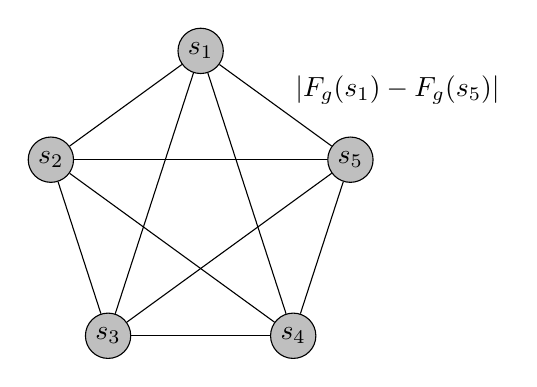
\begin{tikzpicture}
        
        % Define the number of nodes
        \def\n{5}  % Change this for more nodes
        \def\radius{2cm}
        
        % Place nodes in a circular pattern
        \foreach \i in {1,...,\n} {
            \node[draw,circle, fill=gray!50, inner sep=2pt, minimum size=15pt] (s\i) at ({(360/\n * (\i-1))+90}:\radius) {$s_{\i}$};
        }
        
        % Connect every node to every other node
        \foreach \i in {1,...,\n} {
            \foreach \j in {1,...,\n} {
                \ifnum\i<\j
                    \draw (s\i) -- (s\j);
                \fi
            }
        }
        \node (node) at (2.5,1.5) {$|F_g(s_1)-F_g(s_5)|$};
    \end{tikzpicture}
    \end{figure}
    
\end{frame}
\begin{frame}{Búsquedas locales y búsquedas basadas en poblaciones}
    \begin{block}{Búsqueda local}
        Un algoritmo de \alert{búsqueda local} es un algoritmo que comienza en una configuración $s_0\in \mathcal{S}$ y busca una solución moviéndose en el paisaje de adecuación a configuraciones vecinas.
    \end{block}
    \vspace{0.5cm}
    \begin{block}{Búsqueda basada en poblaciones}<2->
        Los algoritmos de \alert{búsqueda basada en poblaciones} de $k>2$ individuos son un tipo de algoritmo que comienza en un conjunto de configuraciones $S$ llado población y explora el, ahora hipergrafo, del paisaje de adecuación.
    \end{block}
\end{frame}

\section{Algoritmos genéticos}

\section{Algoritmos meméticos}

\section{Problemas de rutas}

\section{Algoritmo memético para el MC-TTRP}

\section{Pruebas y resultados}

\begin{frame}{Conclusión}
    
\end{frame}
\end{document}